\documentclass[aspectratio=169]{beamer}
\usepackage[utf8]{inputenc}
\usepackage[T1]{fontenc}
\usepackage{graphicx}
\usepackage{tikz}
\usepackage{booktabs}
\usepackage{colortbl}
\usepackage{amsmath}

% Theme and color
\usetheme{Madrid}
\usecolortheme{default}

% Custom colors
\definecolor{primary}{RGB}{0, 102, 204}
\definecolor{accent}{RGB}{220, 50, 50}
\setbeamercolor{structure}{fg=primary}
\setbeamercolor{title}{fg=white, bg=primary}
\setbeamercolor{frametitle}{fg=white, bg=primary}

% Remove navigation symbols
\setbeamertemplate{navigation symbols}{}

% Slide numbers
\setbeamertemplate{footline}[frame number]

% Metadata
\title[Short Title]{Full Presentation Title}
\subtitle{Subtitle or Context}
\author{Author Name}
\institute{Organization or University}
\date{\today}

\begin{document}

% --- TITLE SLIDE ---
\begin{frame}
\titlepage
\end{frame}

% --- OUTLINE ---
\begin{frame}{Outline}
\tableofcontents
\end{frame}

% --- SECTION 1 ---
\section{Introduction}

\begin{frame}{Problem Statement}
    \begin{itemize}
        \item First key point about the problem
        \item Second key point
        \item Third key point with \textcolor{accent}{\textbf{emphasis}}
    \end{itemize}

    \vspace{1em}
    \begin{block}{Key Insight}
        A highlighted block with an important insight or takeaway.
    \end{block}
\end{frame}

\begin{frame}{Background}
    \begin{columns}[T]
        \column{0.5\textwidth}
        \textbf{Left Column}
        \begin{itemize}
            \item Point A
            \item Point B
            \item Point C
        \end{itemize}

        \column{0.5\textwidth}
        \textbf{Right Column}
        \begin{itemize}
            \item Point D
            \item Point E
            \item Point F
        \end{itemize}
    \end{columns}
\end{frame}

% --- SECTION 2 ---
\section{Method}

\begin{frame}{Our Approach}
    \begin{enumerate}
        \item Step one of the approach
        \item Step two of the approach
        \item Step three of the approach
    \end{enumerate}

    \vspace{1em}
    Key equation:
    \[
        f(x) = \sum_{i=1}^{n} w_i \cdot x_i + b
    \]
\end{frame}

\begin{frame}{Architecture Overview}
    \centering
    % Placeholder for architecture diagram
    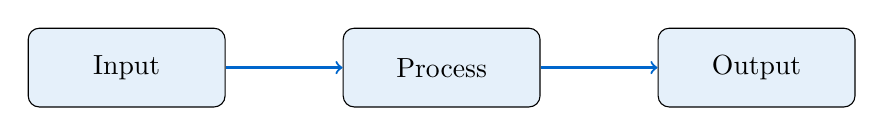
\begin{tikzpicture}[
        box/.style={draw, rounded corners, fill=primary!10, minimum width=2.5cm, minimum height=1cm, align=center},
        arrow/.style={->, thick, primary}
    ]
        \node[box] (input) at (0,0) {Input};
        \node[box] (process) at (4,0) {Process};
        \node[box] (output) at (8,0) {Output};
        \draw[arrow] (input) -- (process);
        \draw[arrow] (process) -- (output);
    \end{tikzpicture}

    \vspace{1em}
    {\small Simplified architecture diagram.}
\end{frame}

% --- SECTION 3 ---
\section{Results}

\begin{frame}{Experimental Results}
    \centering
    \begin{tabular}{lccc}
        \toprule
        \textbf{Method} & \textbf{Metric 1} & \textbf{Metric 2} & \textbf{Metric 3} \\
        \midrule
        Baseline A & 85.2 & 83.1 & 12.3 \\
        Baseline B & 87.5 & 85.4 & 15.7 \\
        \rowcolor{primary!10}
        \textbf{Ours} & \textbf{91.3} & \textbf{89.8} & \textbf{14.2} \\
        \bottomrule
    \end{tabular}
\end{frame}

\begin{frame}{Key Findings}
    \begin{alertblock}{Finding 1}
        An important finding with implications.
    \end{alertblock}

    \begin{exampleblock}{Finding 2}
        A supporting finding with practical examples.
    \end{exampleblock}

    \begin{block}{Finding 3}
        Additional context and nuance.
    \end{block}
\end{frame}

% --- SECTION 4 ---
\section{Conclusion}

\begin{frame}{Summary}
    \textbf{What we did:}
    \begin{itemize}
        \item Contribution 1
        \item Contribution 2
        \item Contribution 3
    \end{itemize}

    \vspace{1em}
    \textbf{Future work:}
    \begin{itemize}
        \item Direction 1
        \item Direction 2
    \end{itemize}
\end{frame}

\begin{frame}
    \centering
    \vspace{2cm}
    {\Huge\textcolor{primary}{Thank You}}

    \vspace{1em}
    {\large Questions?}

    \vspace{2em}
    {\small author@email.com}
\end{frame}

\end{document}
